\begin{figure*}[!tb]
	\centering
	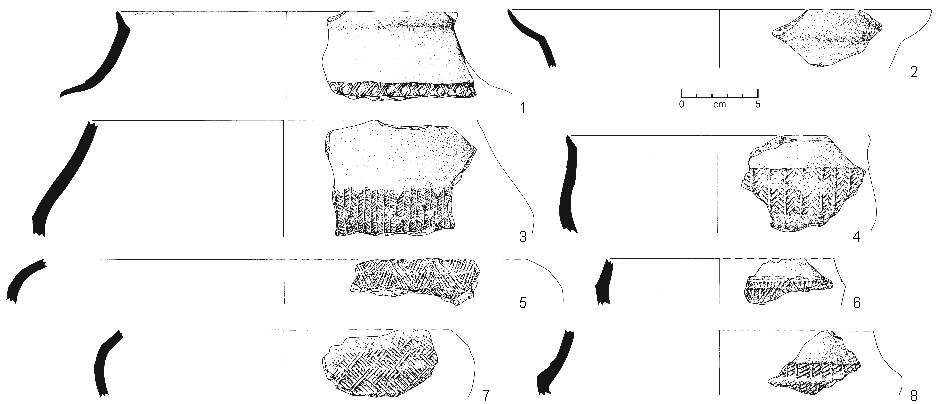
\includegraphics[width=\textwidth]{fig/MBJ-Typen.pdf}
	\caption{Mbenja-Gruppe: Typvertreter.\\1:~Taf.~64.10; 2:~Taf.~65.5; 3:~Taf.~67.16; 4:~Taf.~67.17; 5:~Taf.~59.14; 6:~Taf.~64.13; 7:~Taf.~67.22; 8:~Taf.~64.12.}
	\label{fig:MBJ_Typverteter}
\end{figure*}

\begin{figure*}[!tb]
	\centering
	\begin{subfigure}[t]{\columnwidth}
		\centering
		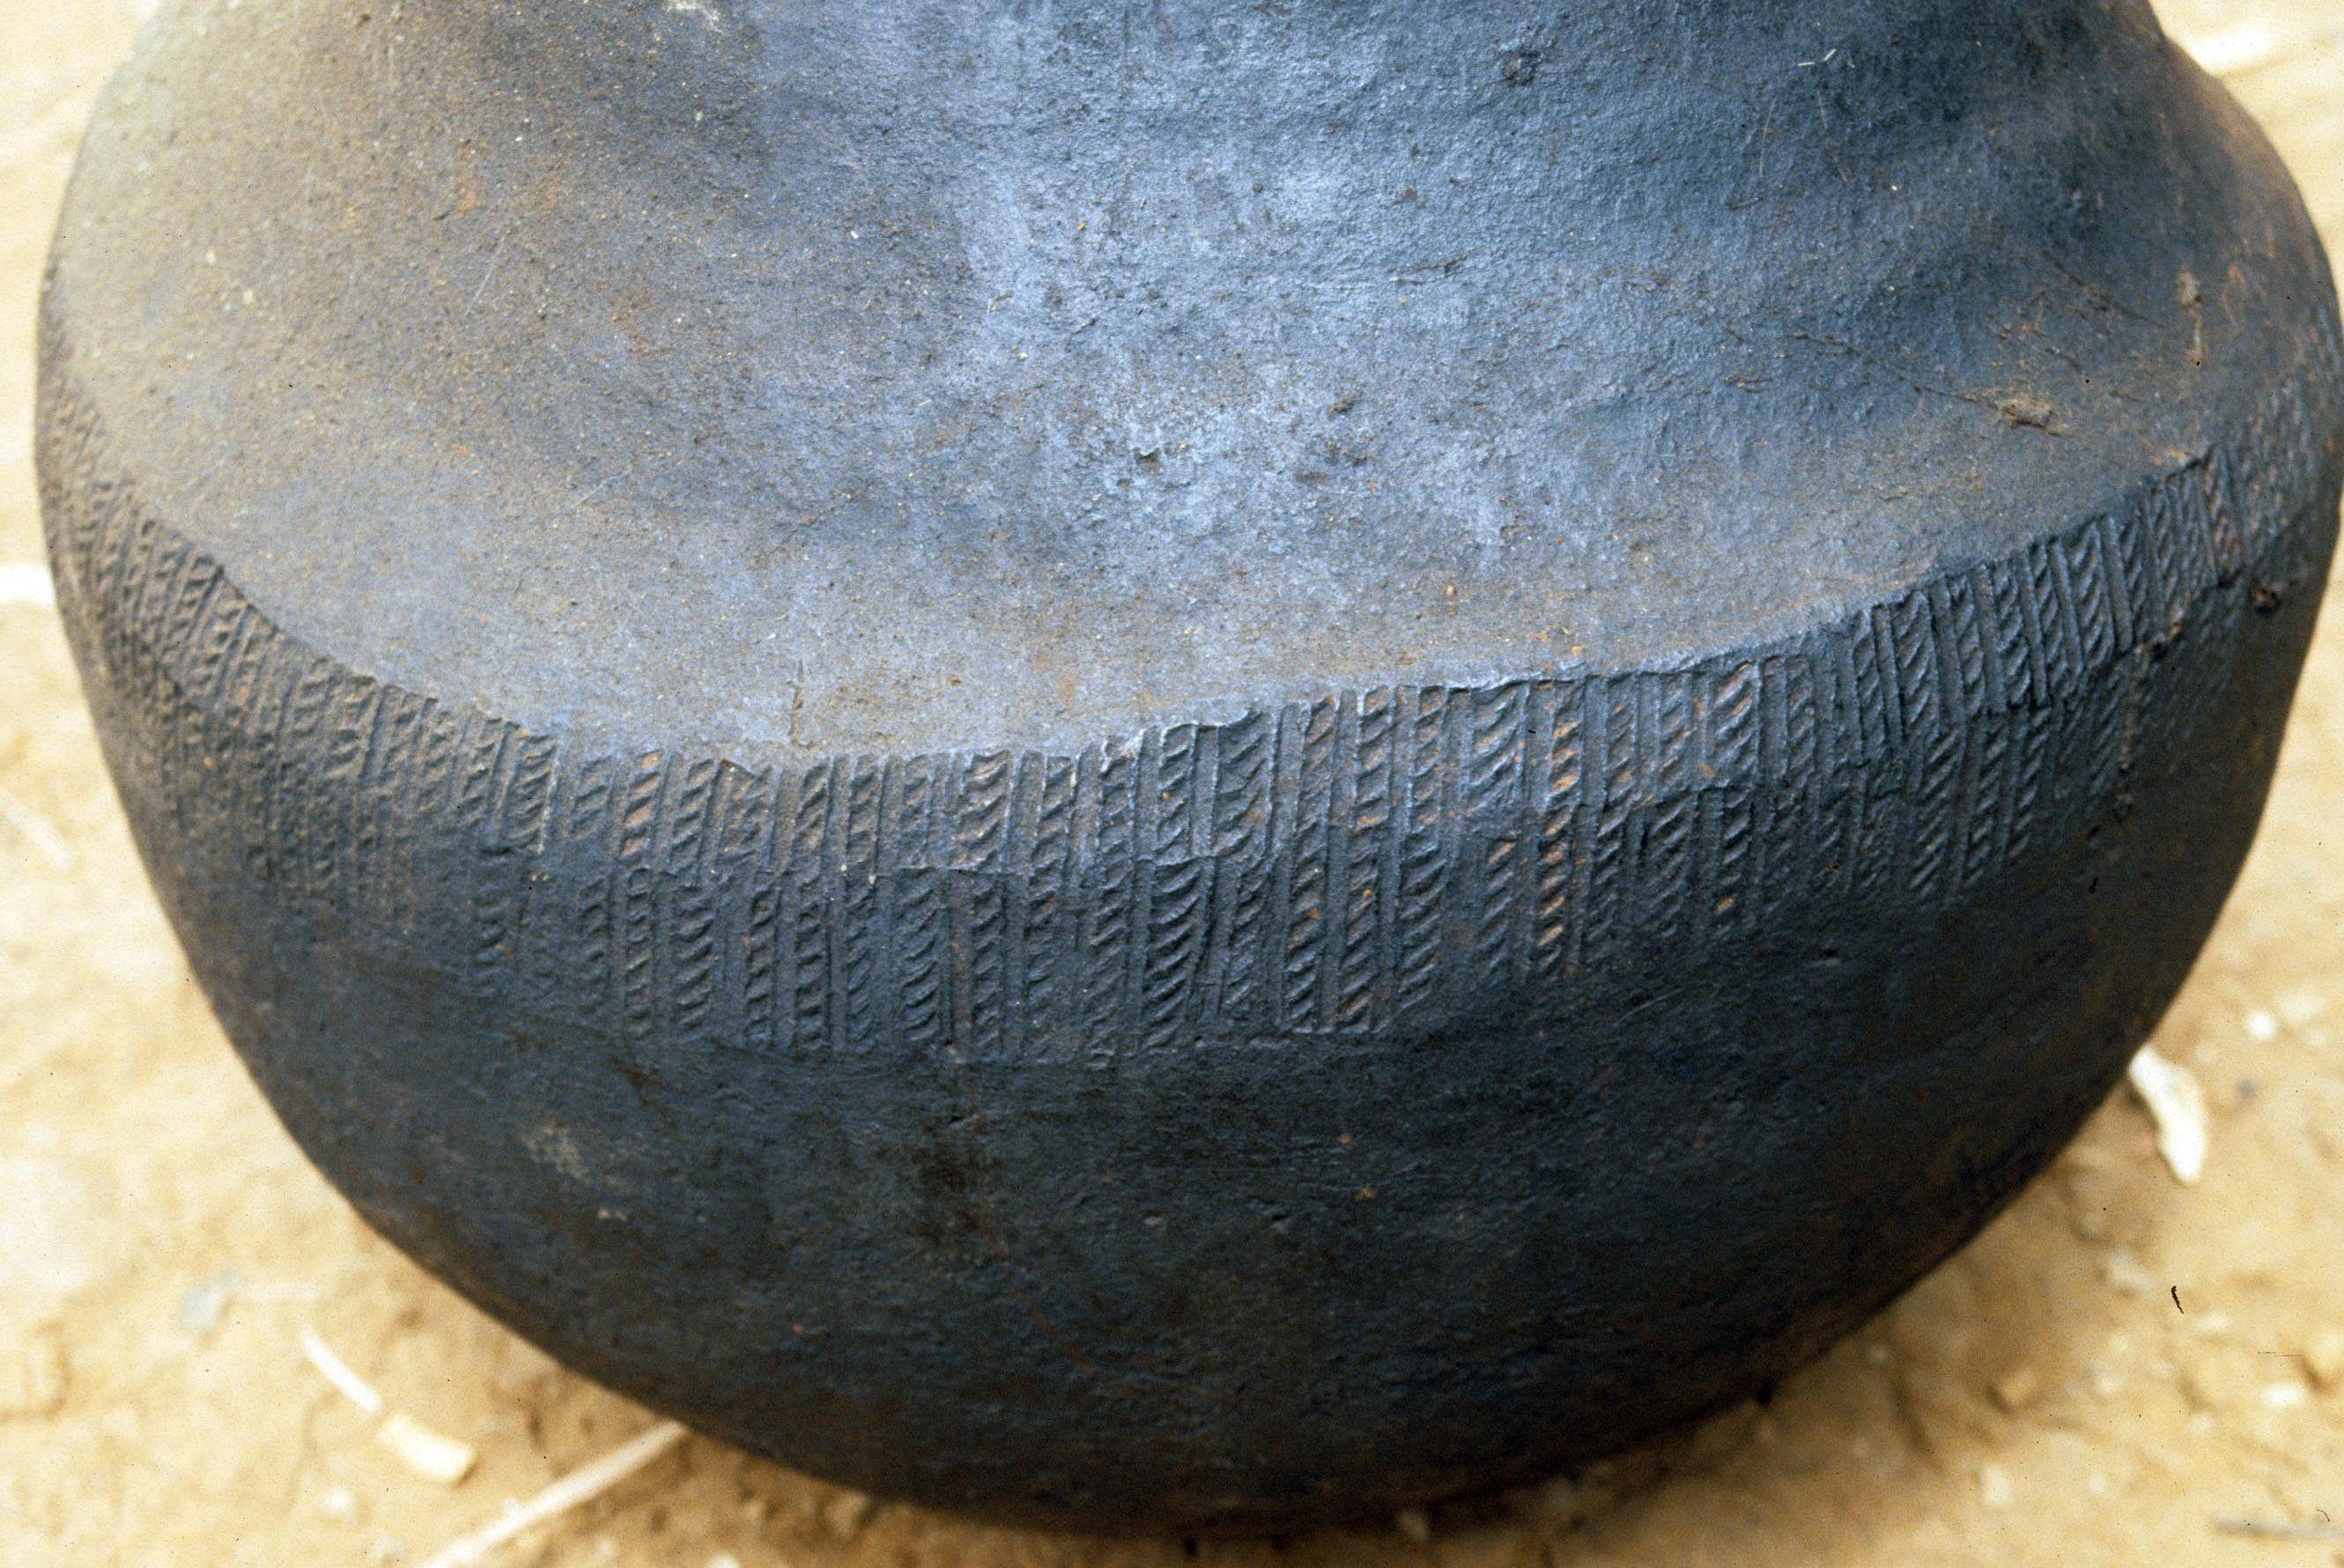
\includegraphics[width = \columnwidth]{fig/MBJ87_Roulettekeramik_E87-010-27.jpg}
		\caption{Bauchiger Topf (Typ~C) mit Schnitzroulette (einzelnes Band) am Bauch-/Schulter-Umbruch.}
		\label{fig:MBJ87_Roulettekeramik_E87-010-27}
	\end{subfigure}\hfill
	\begin{subfigure}[t]{\columnwidth}
		\centering
		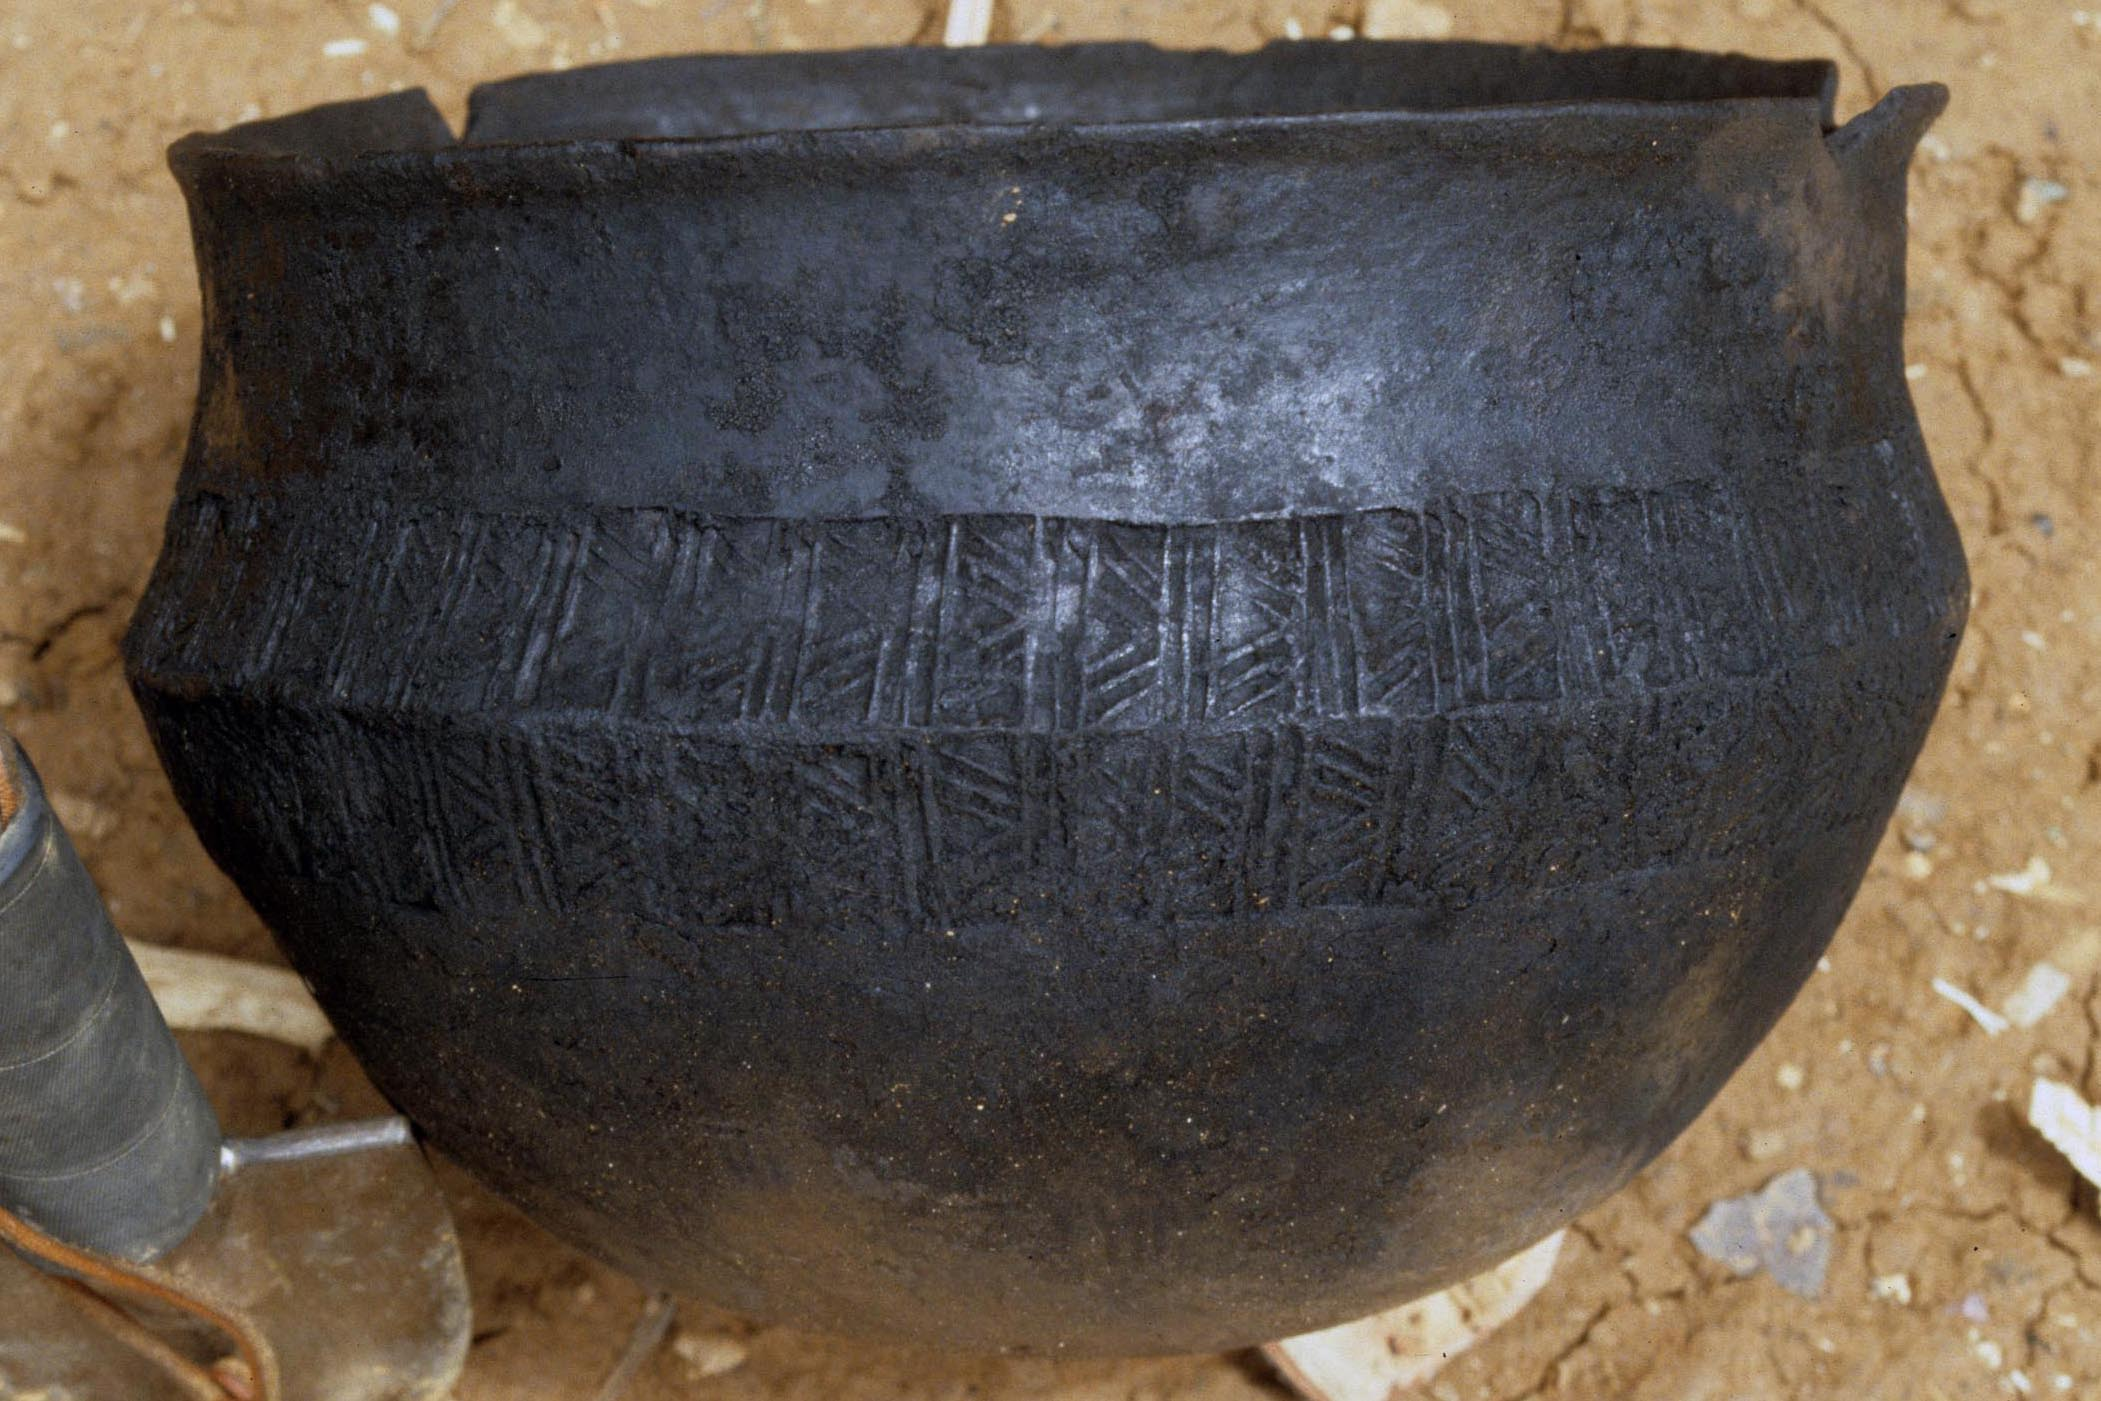
\includegraphics[width = \columnwidth]{fig/MBJ87_Roulettekeramik_E87-010-25.jpg}
		\caption{Rundbodige Schalen (Typ~F2) mit Bauchknick und ausbiegendem Rand.}
		\label{fig:MBJ87_Roulettekeramik_E87-010-25}
	\end{subfigure}
	\caption{Mbenja (Fpl.~277): Keramikgefäße (Fotos: M.~K.~H.~Eggert, 1987).}
	\label{fig:MBJ87_Roulettekeramik}
\end{figure*}

\subsubsection{Mbenja-Gruppe}\label{sec:MBJ-Gr}

Die Mbenja-Gruppe beschreibt die rezente Keramik im Bereich des oberen \mbox{Sangha} sowie entlang des prospektierten Abschnitts der \mbox{Ngoko}. Dieser Stilgruppe zugeordnete Stücke wurden an insgesamt 16 verschiedenen Fundplätzen nachgewiesen, wobei das am mittleren \mbox{Sangha} gelegene Pikunda (Fpl.~255) den südlichsten Fundpunkt der Verbreitung markiert (Abb.~\ref{fig:MBJ_Verbreitung}). Material der Mbenja-Gruppe fand sich weiter stromaufwärts am \mbox{Sangha} wie am \mbox{Ngoko} bis zu den jeweiligen Endpunkten der Befahrung von 1987 in Bomasa (Fpl.~274a) sowie Yengo (Fpl.~282). Im untersuchten Material finden sich weder vollständige Gefäße noch Bodenstücke, die der Mbenja-Gruppe zugerechnet werden können. Das Gros des zuweisbaren Materials, insgesamt 102 individuell aufgenommene GE sowie 52 ausgezählt erfasste Scherben, besteht aus Wandungsstücken (84\,\%).  Randscherben machen mit 16\,\% lediglich einen kleinen Teil des Fundguts aus. Aufgrund dieser Einschränkung sowie der noch zu beleuchtenden Ähnlichkeiten von Gefäßformen und Verzierungen zwischen den Stilen Pandama (Kap.~\ref{sec:PDM-Gr}) und Mbenja konnten lediglich 57\,\% der Stücke sicher dem Mbenja-Stil zugeordnet werden. Zusammengenommen besteht das Material der Mbenja-Gruppe aus 161 individuellen GE. Die Bezeichnung der Stilgruppe gründet auf zwei in Mbenja am \mbox{Ngoko} (Fpl.~277) fotografierten Gefäßen (Abb.~\ref{fig:MBJ87_Roulettekeramik}). 

\paragraph{Technologische Merkmale}\hspace{-.5em}|\hspace{.5em}%
Die Keramik der Mbenja-Gruppe zeichnet sich nicht durch ein spezifisches \textit{Fabric} aus, vielmehr ist eine starke Heterogenität zu beobachten. Am häufigsten sind die \textit{Fabrics} 4 (39\,\%), 3 (23\,\%) sowie 5 (17\,\%) und 7 (13\,\%) vertreten. Allen \textit{Fabrics} der Mbenja-Keramik ist gemeinsam, dass sie einen hohen Anteil nichtplastischer Partikel aufweisen. Zusammengenommen mehr als 70\,\% aller Scherben weisen Anteile an nichtplastischen Partikeln von mehr als 15--20\,\% auf. Eine sehr ähnliche Verteilung ergibt sich mit Blick auf die Größe der nichtplastischen Partikel. Fast 67\,\% aller Stücke weisen Partikel der Größenklassen \textit{coarse} (47\,\%) und \textit{very coarse} (22\,\%) auf. Bei diesen Partikeln handelt es sich vor allem um heterogene Mischungen aus Quarzsand. Nur einzelne Stücke enthalten nichtplastische Partikel, die als Lateritfragmente angesprochen werden können. Während lediglich bei 39\,\% der Stücke die Brennfarbe des genutzten Tons angesprochen werden konnte, 24\,\% deuten auf rotbrennenden und 15\,\% auf weißbrennende Tone hin, weist ein großer Teil der Stücke eine graue, beige oder schwarze Färbung auf, welche keinen unmittelbaren Rückschluss auf die Brennfarbe des genutzten Tons zulässt. Die Oberflächen der Scherben sind größtenteils glatt (54\,\%) oder leicht rau (35\,\%). Die Wandungsdicke schwankt zwischen \mbox{4--10\,mm}.

\begin{figure*}[p]
	\centering
	\includegraphics[width=\textwidth]{fig/MBJ_Verbreitung.pdf}
	\caption{Mbenja-Gruppe: Verbreitung.}
	\label{fig:MBJ_Verbreitung}
\end{figure*}


\paragraph{Formen}\hspace{-.5em}|\hspace{.5em}%
Während bei 31~GE die Gefäßform angesprochen werden konnte, fiel aufgrund der starken Fragmentierung der Stücke sowie des Umstandes, dass es sich größtenteils um Wandungsfragmente handelt, die Ansprache in lediglich 30\,\% aller Fälle sicher aus. Die am häufigsten angetroffene Gefäßform sind bauchige Gefäße mit deutlich ausgeprägter Gefäßschulter vom Typ C2, die 55\,\% aller identifizierten Gefäßformen ausmachen (Abb.~\ref{fig:MBJ_Typverteter}.1, 5, 7; Abb.~\ref{fig:MBJ87_Roulettekeramik_E87-010-27}). Gefäße mit geschweifter Wandung und schwach ausgeprägter Gefäßschulter vom Typ C1 machen 13\,\% der Formen aus. Flachere Gefäße mit deutlichem Bauchknick vom Typ F2 sind zu 16\,\% vertreten (Abb.~\ref{fig:MBJ_Typverteter}.6, 8; Abb.~\ref{fig:MBJ87_Roulettekeramik_E87-010-25}). Weitere Formen sind nur in wenigen einzelne Individuen belegt, so etwa leicht bauchige Gefäße vom Typ E2, hohe Gefäße mit Bauchknick des Typs F1 sowie rundbauchige Schalen vom Typ I1. Die GE der Mbenja-Gruppe zeigen vornehmlich konvexe Gefäßbäuche (82\,\%). Etwa 18\,\% der Stücke weisen jedoch einen mehr oder weniger deutlich ausgeprägten Profilknick im Bauchbereich auf (Abb.~\ref{fig:MBJ_Typverteter}.6--8, \ref{fig:MBJ87_Roulettekeramik_E87-010-25}). Die Ränder der Mbenja-Keramik sind regelhaft ausbiegend. Das Gros bilden einfach ausbiegende, gerade Ränder des Typs B1 (73\,\%). Daneben finden sich auch die bereits bei der Pandama-Gruppe (Kap.~\ref{sec:PDM-Gr}) beobachteten konkav ausbiegenden Ränder des Typs B3 (Abb.~\ref{fig:MBJ_Typverteter}.2). Die Ausgestaltung des Mündungsabschlusses zeigt eine größere Variabilität, obschon spitz ausgeformte Randlippen vom Typ M2 mit 48\,\% deutlich dominieren. Es kommen aber auch runde (M1; 29\,\%) sowie gerade abgestrichene Randabschlüsse (M3; 10\,\%) vor. Fast ein Drittel aller Gefäßhälse ist auffällig lang ausgearbeitet. Bestimmend sind Kegelhälse (Abb.~\ref{fig:MBJ_Typverteter}.1, 3), wobei auch zylindrische oder konkave Ausformungen vorkommen. Die Gefäßschultern sind regelhaft schräg (27\,\%) oder konvex (40\,\%) ausgearbeitet. Über die Ausprägung der Gefäßböden kann keine Aussage gemacht werden, da keine Bodenstücke vorliegen, die der Mbenja-Keramik zugewiesen werden können. Lediglich die in Mbenja am \mbox{Ngoko} (Fpl.~277) fotografierte Schale zeigt einen runden Gefäßboden vom Typ B1 (Abb.~\ref{fig:MBJ87_Roulettekeramik_E87-010-25}).
 
\paragraph{Verzierungen}\hspace{-.5em}|\hspace{.5em}%
Die Keramik der Mbenja-Gruppe ist vornehmlich durch ihre Rouletteverzierung bestimmt. Zusammengenommen sind 84\,\% aller beobachteten Verzierungselemente Schnitzrouletteverzierungen. Innerhalb dieser macht die \textit{Tannenzweig}-Schnitzroulette-Variante 21.12 (Tab.~\ref{tab:Verzierungselemente}) 62\,\% aus. Bereits deutlich seltener kommen die Schnitzroulette-Varianten 21.8 (22\,\%), 21.6 (8\,\%), 21.7 (5\,\%) sowie 21.11 (3\,\%) vor. Insgesamt entfallen 7\,\% der Verzierungen auf ein flächiges Muster, bei dem es sich um Mattenabdruck handeln könnte (Tab.~\ref{tab:Verzierungselemente}: 20.1). Die häufigsten Verzierungselemente, bei denen es sich nicht um Rouletteverzierung handelt, sind Reihen aus diagonal gestellten, kleinen Eindrücken (Tab.~\ref{tab:Verzierungselemente}: 04.12) sowie lange, bogenförmige Eindrücke (Tab.~\ref{tab:Verzierungselemente}: 04.19). Diese machen jeweils weniger als 3\,\% der aufgenommenen Verzierungselemente aus. Die Keramik der Mbenja-Gruppe ist vornehmlich im Bereich des Gefäßbauches (56\,\%) sowie der Gefäßschulter (33\,\%) verziert. Eine Verzierung des Unterteils der Gefäße ist in keinem Fall beobachtet worden. Die in Mbenja am \mbox{Ngoko} (Fpl.~277) fotografierten Gefäße (Abb.~\ref{fig:MBJ87_Roulettekeramik}) illustrieren das Verzierungsschema der Mbenja-Keramik in besonderem Maße. Beide Stücke enthalten neben schmalen Roulette-Bändern im Bereich des Übergangs von der Gefäßschulter zum Gefäßbauch (Abb.~\ref{fig:MBJ87_Roulettekeramik_E87-010-27}) sowie auf dem Gefäßbauch beziehungsweise Bauchknick (Abb.~\ref{fig:MBJ87_Roulettekeramik_E87-010-25}) keine Verzierungen. Das Charakteristikum der fast ausschließlichen Schnitzrouletteverzierung unterscheidet die Mbenja-Keramik von der sich durch die Kombination von Verzierungselementen auszeichnenden Pandama-Keramik (Kap.~\ref{sec:PDM-Gr}). 


\paragraph{Datierung}\hspace{-.5em}|\hspace{.5em}%
Für die Keramik der Mbenja-Gruppe liegen keine absoluten Datierungen vor. Die Dokumentation der Nutzung der Keramik im Jahr 1987 belegt die chronologische Stellung dieser keramischen Stilgruppe am Ende der erarbeiteten Sequenz (Abb.~\ref{fig:Chronologiesystem}). Die Keramik der Mbenja-Gruppe bildet das rezente keramische Inventar am oberen \mbox{Sangha} sowie dem \mbox{Ngoko} ab.


\paragraph{Verbreitung}\hspace{-.5em}|\hspace{.5em}%
Das Verbreitungsgebiet der Mbenja-Keramik ist auf den Oberlauf des \mbox{Sangha} sowie den befahrenen Abschnitt des \mbox{Ngoko} begrenzt (Abb.~\ref{fig:MBJ_Verbreitung}).\footnote{Auf Basis von Fundfotografien lassen sich auch Funde aus dem am oberen \mbox{Sangha} gelegenen Mboua Mboua unter Vorbehalt der Mbenja-Gruppe zuordnen (\textsc{Gillet} 2013: 114 Abb.~42). Siehe auch Kap.~\ref{sec:PKM-Gr}.} Die südlichste sicher der Mbenja-Gruppe zugerechnete GE findet sich in Molanda am mittleren \mbox{Sangha} (Fpl.~258). Etwas weiter südlich, in Pikunda (Fpl.~255), fanden sich ebenfalls möglicherweise der Mbenja-Gruppe zuzurechnende Stücke. Das erfasste Verbreitungsgebiet ist stromauf beziehungsweise nach Norden und Westen durch die Grenzen der Prospektion und damit des Arbeitsgebietes markiert. Entlang des \mbox{Sangha} wurden in Bonda (Fpl.~272) die nördlichsten Mbenja-Scherben gefunden, während der westlichste Endpunkt der beobachteten Verbreitung am \mbox{Ngoko} in Ngama (Fpl.~281) liegt. Aussagen über die weitere Verbreitung der Mbenja-Keramik in Richtung Kamerun oder der Zentralafrikanischen Republik können nicht getroffen werden. 	
